\subsubsection{User Profile}
\begin{figure}[H]
	\begin{subfigure}{0.80\linewidth}
		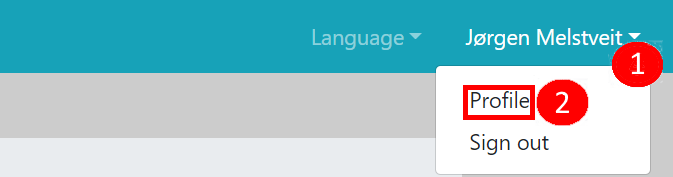
\includegraphics[width=\linewidth]{userManual/client/userProfile/accessUserProfile}
		\caption{}
		\label{fig:accessUserProfile}	
	\end{subfigure}
	\begin{subfigure}{0.80\linewidth}
		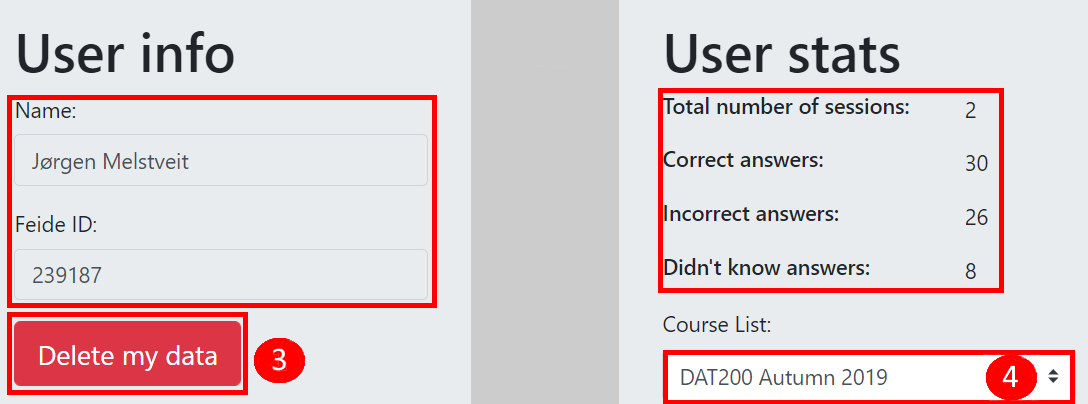
\includegraphics[width=\linewidth]{userManual/client/userProfile/profile}
		\caption{}
		\label{fig:profilePage}
	\end{subfigure}
\end{figure}

\begin{userManualItemlist}
	\item[Step I.] You need to be signed in to your Feide Account to access your user account. 
	\item[Step II.] Click the button (1) with your Feide name on the navigation bar. (Figure: \ref{fig:accessUserProfile})
	\item[Step III.] Click "Profile" button (2). (Figure: \ref{fig:accessUserProfile})
	\item[Step IV.] View user info. The user info contains the Feide username and Feide name. (Figure: \ref{fig:profilePage})
	\item[Step V.] Click the button (3) labeled "Delete my data" if you want to delete your user data on the application. This includes your old session data. (Figure: \ref{fig:profilePage})
	\item[Step VI.] View user stats. The stats includes your total number of sessions, the total amount of questions you answered correctly, the total amount of questions you answered incorrectly and how many times you answered "I don't know". (Figure: \ref{fig:profilePage})
	\item[Step VII.] Choose the course you want to view session data for (4). If you participated in a session corresponding to the selected course, a list of sessions will appear. (Figure: \ref{fig:profilePage})
	\item[Step VIII.] Click on the selected session you want to view your answers for.
\end{userManualItemlist}